%%%%%%%%%%%%%%%%%%%%%%%%%%%%%%%%%%%%%%%%%%%%%%%%%%%%%%%%%%%%%%%%%%%%%%%%%%%%%%%%
%2345678901234567890123456789012345678901234567890123456789012345678901234567890
%        1         2         3         4         5         6         7         8

\documentclass[letterpaper, 10 pt, conference]{ieeeconf}  % Comment this line out if you need a4paper

%\documentclass[a4paper, 10pt, conference]{ieeeconf}      % Use this line for a4 paper

\IEEEoverridecommandlockouts                              % This command is only needed if 
                                                          % you want to use the \thanks command

\overrideIEEEmargins                                      % Needed to meet printer requirements.

%In case you encounter the following error:
%Error 1010 The PDF file may be corrupt (unable to open PDF file) OR
%Error 1000 An error occurred while parsing a contents stream. Unable to analyze the PDF file.
%This is a known problem with pdfLaTeX conversion filter. The file cannot be opened with acrobat reader
%Please use one of the alternatives below to circumvent this error by uncommenting one or the other
%\pdfobjcompresslevel=0
%\pdfminorversion=4

% See the \addtolength command later in the file to balance the column lengths
% on the last page of the document

% The following packages can be found on http:\\www.ctan.org
\usepackage{graphics} % for pdf, bitmapped graphics files
\usepackage{epsfig} % for postscript graphics files
\usepackage{mathptmx} % assumes new font selection scheme installed
\usepackage{times} % assumes new font selection scheme installed
\usepackage{amsmath} % assumes amsmath package installed
\usepackage{amssymb}  % assumes amsmath package installed
\usepackage{xcolor}

\newcommand{\aku}[1]{\textcolor{blue}{AS: #1}}

\title{\LARGE \bf
FoundationPose vs.\ EKF-Based Stereo Pose Tracking for Manipulator Visual Servoing
}

\author{Akanksha Singal and Sidd Vohra\\
Carnegie Mellon University\\
{\tt\small \{asingal2, svohra\}@andrew.cmu.edu}
}

\begin{document}

\maketitle
\thispagestyle{empty}
\pagestyle{empty}


%%%%%%%%%%%%%%%%%%%%%%%%%%%%%%%%%%%%%%%%%%%%%%%%%%%%%%%%%%%%%%%%%%%%%%%%%%%%%%%%
\begin{abstract}
Robust visual servoing is critical for autonomous manipulation in unstructured environments such as warehouses, homes etc. Visual servoing requires accurate estimation of the relative pose between the robot end-effector and the target grasp point. We compare two fundamentally different approaches to 6DoF pose estimation in an iterative visual servoing loop: FoundationPose, a learning-based method that produces per-frame pose estimates from RGB-D input, and an Extended Kalman Filter (EKF) based pose tracker that maintains a probabilistic belief over the camera state across time. We evaluate both methods in simulation, measuring convergence, accuracy, robustness to noise, and runtime in the context of iterative pose-based visual servoing. Our goal is to characterize the trade-offs between a memoryless, high-capacity model and a stateful, uncertainty-aware classical estimator when pose errors compound over a closed-loop trajectory.
\end{abstract}


%%%%%%%%%%%%%%%%%%%%%%%%%%%%%%%%%%%%%%%%%%%%%%%%%%%%%%%%%%%%%%%%%%%%%%%%%%%%%%%%
% \section{INTRODUCTION \& IMPACT}

% Reliable visual servoing is fundamental for autonomous robotic manipulation in applications such as warehouse automation, household robotics, and surgical. Classical visual servo pipelines depend heavily on accurate pose estimation from geometric pipelines that often degrade in low-texture, cluttered, or partially occluded environments. This project investigates stereo pose tracking methods for visual servoing, combining classical state-estimation approaches (EKF-based tracking) with modern learning-based pose estimators (e.g., FoundationPose). The outcome will provide insights into the trade-offs between model-based and learning-based perception for closed-loop control and contribute toward more robust manipulation systems in unstructured environments.

% Visual servoing uses visual feedback to control a robot's motion toward a goal pose. Pose-based visual servoing (PBVS) relies on accurate 6DoF camera pose estimation at each iteration. Errors in pose estimation propagate through the control loop, potentially causing divergence or inefficient trajectories.

% Recent foundation models such as FoundationPose~\cite{foundationpose} achieve strong single-frame pose accuracy on standard benchmarks. However, these models are memoryless: each frame is processed independently with no temporal context. In contrast, the Extended Kalman Filter (EKF) maintains a state estimate and covariance across time, naturally handling noisy measurements through sequential Bayesian estimation.

% This project provides a systematic comparison of these two paradigms in a closed-loop visual servoing setting, where the key question is not just per-frame accuracy but how well each method supports iterative convergence to a goal pose under realistic conditions.


% Most evaluations of pose estimation methods focus on single-frame accuracy on static benchmarks. In practice, pose estimates are consumed by downstream control loops where errors accumulate. Understanding the behavior of learning-based vs.\ filtering-based methods in this setting has direct implications for practitioners designing visual servoing systems. Specifically, we aim to answer: does the EKF's uncertainty tracking and temporal smoothing offer meaningful advantages over a powerful per-frame estimator, and under what degraded conditions does one approach fail before the other?
\section{INTRODUCTION \& IMPACT}

Reliable visual servoing is fundamental to autonomous robotic manipulation in applications such as warehouse automation, household robotics, and surgical assistance. Classical visual servo pipelines rely heavily on accurate pose estimation obtained from geometric reconstruction pipelines. However, these pipelines often degrade in low-texture, cluttered, or partially occluded environments, leading to unstable or inefficient closed-loop behavior. This project investigates stereo pose tracking methods for visual servoing by comparing classical state-estimation approaches (EKF-based tracking) with modern learning-based pose estimators (e.g., FoundationPose). The goal is to understand how perception design choices impact downstream control performance and to advance more robust manipulation systems for unstructured environments.

Visual servoing uses visual feedback to regulate robot motion toward a desired goal pose. In particular, pose-based visual servoing (PBVS) depends critically on accurate 6-DoF pose estimates at every control iteration. Errors in pose estimation propagate directly through the control loop and can result in slow convergence, oscillatory behavior, or even divergence. Consequently, evaluating perception modules solely based on single-frame pose accuracy is insufficient for understanding their effectiveness in closed-loop robotic systems.

Recent foundation models such as FoundationPose~\cite{foundationpose} demonstrate strong single-frame pose accuracy on standard benchmarks. However, these models are inherently memoryless, processing each frame independently without leveraging temporal consistency. In contrast, the Extended Kalman Filter (EKF) maintains a recursive state estimate and covariance over time, enabling principled uncertainty handling and temporal smoothing through sequential Bayesian estimation.

This project provides a systematic closed-loop comparison of these two paradigms for stereo visual servoing. Rather than focusing only on per-frame pose accuracy, we evaluate how each approach supports iterative convergence to a desired goal pose under realistic operating conditions. Most existing evaluations of pose estimation methods emphasize static, open-loop benchmarks, whereas in practice pose estimates are consumed by downstream controllers where errors compound over time.

Understanding the relative strengths of learning-based versus filtering-based pose tracking in this closed-loop setting has direct implications for practitioners designing visual servo systems. Specifically, we aim to answer the following question: \emph{does the EKF's temporal filtering and uncertainty propagation provide meaningful advantages over a high-capacity per-frame pose estimator, and under what degraded visual conditions does one approach fail before the other?}

\section{NOVELTY}

While FoundationPose has been benchmarked extensively on datasets like BOP and YCB-Video, we are not aware of a direct comparison with EKF-based tracking in an iterative servoing loop. 
% The novel contribution of this project is evaluating these methods not on static pose accuracy but on closed-loop servoing performance, including convergence rate, path efficiency, and robustness under systematic perturbations (noise, occlusion, lighting). This comparison highlights trade-offs that do not surface in standard benchmarking.
The key novelty of this project lies in evaluating stereo pose tracking methods through the lens of control performance rather than standalone perception accuracy. Specifically, we integrate both EKF-based stereo tracking and FoundationPose into a unified pose-based visual servoing (PBVS) pipeline and assess their impact on iterative convergence to a goal pose.

We evaluate performance using control-relevant metrics including convergence rate, time to convergence, path efficiency, and robustness under systematic degradations such as measurement noise, partial occlusion, and lighting variation. This study exposes perception–control trade-offs that are not visible in standard pose estimation benchmarks and provides practical guidance for designing robust visual servoing systems.

\section{METHODS}

We will use the following methods and concepts from the course:

\textbf{Extended Kalman Filter:} We implement an EKF for 6DoF pose tracking. The state vector contains the camera pose (position and orientation). The motion model predicts the next pose given the servoing control command. The measurement model incorporates depth-based or feature-based observations to correct the predicted state. The EKF linearizes both models around the current estimate and propagates the covariance matrix, providing uncertainty estimates alongside pose estimates.

\textbf{Rigid Body Transformations and Rotations:} Both methods require reasoning about SE(3) transformations. We will represent rotations carefully using rotation matrices and handle the manifold structure when computing pose errors and control commands.

\textbf{Least-Squares Pose Estimation:} The EKF measurement update can be understood as a sequential least-squares problem. We will use this connection to analyze the estimator's behavior.

\textbf{Covariance and Uncertainty:} The EKF produces covariance estimates that characterize pose uncertainty. We will analyze how this uncertainty evolves during servoing and compare it against empirical errors from FoundationPose.

\textbf{State-Space Modeling of Nonlinear Systems:} The visual servoing pipeline is formulated in a nonlinear state-space framework. We explicitly model the system dynamics and measurement processes required by the EKF, enabling principled recursive estimation and analysis of error propagation in closed loop.

\section{METRICS FOR SUCCESS}

We will evaluate both methods on:
\begin{enumerate}
    \item \textbf{Final pose error:} Translation (cm) and rotation (degrees) error between the achieved and goal poses after the servoing loop terminates.
    \item \textbf{Convergence rate:} Number of iterations (or time) to reach the goal within a specified tolerance.
    \item \textbf{Path efficiency:} Ratio of actual trajectory length to the geodesic distance on SE(3) between start and goal.
    \item \textbf{Robustness:} Success rate under varying levels of measurement noise, partial occlusion, and lighting changes.
    \item \textbf{Runtime:} Per-iteration inference time for each method.
\end{enumerate}
We propose to evaluate these metrics using Isaac sim environment and real-world experiments (if time allows).

\section{CHALLENGES}

The main technical challenges we anticipate are:

\textbf{Fair comparison:} FoundationPose uses RGB-D and a CAD model as input. The EKF measurement model must be given comparable information (e.g., depth-based correspondences or rendered reference views) to avoid biasing the comparison.

\textbf{EKF tuning:} The EKF's performance depends on process and measurement noise covariance tuning. We need to tune these carefully and report sensitivity.

\textbf{Simulation realism:} We need a rendering pipeline that produces realistic enough images for FoundationPose to work as intended, while also providing ground truth poses for evaluation.

\textbf{Rotation representation:} Properly handling rotations and avoiding singularities in the EKF state update requires care, particularly when computing Jacobians on the SO(3) manifold.

\section{RESOURCES}

\textbf{Software:} FoundationPose (NVIDIA, open-source), OpenCV, NumPy/SciPy for the EKF implementation, PyBullet or Blender for synthetic rendering with ground truth poses.

\textbf{Datasets:} We will use synthetic scenes with known ground truth from Isaacsim simulation. We may additionally evaluate on YCB-Video objects rendered in simulation to test generalization.

\textbf{Compute:} Standard GPU for FoundationPose inference. The EKF runs on CPU. 

\textbf{Hardware:} xARM manipulator with Zed mini camera.

\section{TIMELINE}

\begin{tabular}{l l}
\textbf{Weeks 1-2} & Set up FoundationPose, implement EKF pose \\
 & tracker, validate both on static frames. \\
\textbf{Weeks 3-4} & Build simulated servoing loop, integrate both \\
 & methods, implement PBVS controller. \\
\textbf{Week 5} & Run experiments: noise sweeps, occlusion, \\
 & lighting. Collect metrics. \\
\textbf{Week 6} & Analysis, final writeup, presentation. \\
\end{tabular}

\section{MID TERM DRAFT}

\aku{Our visual servoing pipeline performs real-time object localization in the camera frame using a detect-then-track architecture. In the detection phase, we extract dense patch-level features from both a reference object image and the live scene using DINOv2 (ViT-B/14), compute a cosine similarity map between foreground reference patches and scene patches, threshold and cluster this map to produce a bounding box, and then prompt SAM2 with that box to obtain a precise segmentation mask and low-resolution logits. In subsequent frames, we bypass the expensive DINOv2 feature extraction entirely and instead propagate the previous frame's SAM2 logits as a mask prompt on the new image, achieving 5–10× faster per-frame processing. The tracker monitors SAM2 confidence scores, mask area stability, and periodic frame counts to decide when to fall back to full re-detection. To estimate a grasp-quality target within the localized mask, we run monocular depth estimation (Depth Anything V2) and compute a quality score based on local depth smoothness — combining inverse depth gradient magnitude and local standard deviation — selecting the smoothest, most graspable region as the servo target. The resulting 2D centroid error relative to the image center is then mapped to robot end-effector corrections via a Jacobian estimated through an online optical-flow-based calibration procedure, closing the visual servoing loop.}

\section{Methodology}

 
Our system consists of three subsystems: (1)~a perception module that localises the target object, (2)~a state estimator that filters noisy observations into smooth pose estimates, and (3)~a PBVS controller that converts the estimated pose into robot commands.
We implement variants of subsystem 2 to analyze which gives the better accuracy and overall trajectory.

\subsection{Perception Module: Detect-Then-Track}
 
\textbf{Detection mode} (first frame and re-detection):
Dense patch-level features are extracted from both a reference image and the live scene using DINOv2 (ViT-B/14).
For each scene patch, we compute the mean cosine similarity against all foreground reference patches, yielding a spatial similarity map.
This map is thresholded (at a configurable percentile), morphologically cleaned, and clustered via connected components to produce a bounding box.
The box is used as a prompt for SAM2, which returns an instance segmentation mask and low-resolution logits $\ell \in \mathbb{R}^{1 \times 256 \times 256}$.

\textbf{Tracking mode} (subsequent frames):
The previous frame's SAM2 logits are passed as a \texttt{mask\_input} prompt to SAM2 on the new frame, propagating the segmentation without re-running DINOv2.
This achieves $5$--$10\times$ faster per-frame processing.
Tracking confidence is monitored via the SAM2 prediction score, mask area stability, and a periodic re-detection interval; if any trigger fires, the system reverts to detection mode.
 
The ResNet-18 feature similarity map can be fused with the DINOv2 similarity via a weighted combination for more robust detection

\subsection{EKF-Based Pose Tracker}
\textcolor{red}{need to check then add}

\subsection{PBVS Controller}
Both estimators feed into a common PBVS controller.
For Baseline, we use Image Based Visual Servoing (IBVS) using a calibrated $2 \times 2$ image Jacobian estimated via online optical-flow calibration.

\section{REMAINING WORK}
\begin{itemize}
\item Complete FoundationPose integration into the PBVS loop.
\item Run closed-loop servoing experiments in real world with multiple estimators.
\item Collect metrics: final pose error, convergence rate, path efficiency, robustness under noise/occlusion, and per-frame runtime.
\item Perform EKF noise covariance sensitivity analysis ($\mathbf{Q}$, $\mathbf{R}$ sweeps).
\item Final analysis and writeup.
\end{itemize}

\section{TIMELINE}

\begin{tabular}{l l}
\textbf{Weeks 1-2 } & Implement DINO + SAM \\
(DONE) & pipeline as baseline, \\
& Implement EKF pose \\
\textbf{Weeks 3-4} & Build servoing loop, integrate \\
 (DONE) & both methods, implement PBVS controller \\
 & for real world experiments \\
\textbf{Week 5} & Implement FoundationPose and \\
& Run experiments: noise sweeps, occlusion, \\
& lighting. Collect metrics. \\
\textbf{Week 6} & Analysis, final writeup, presentation. \\
\end{tabular}
 
\begin{figure*}[t]
    \centering

    % Row 1
    
\includegraphics[width=0.24\textwidth]{objects/protein_bar.jpeg}\hfill
    
\includegraphics[width=0.24\textwidth]{objects/baking_mix_box.jpeg}\hfill
    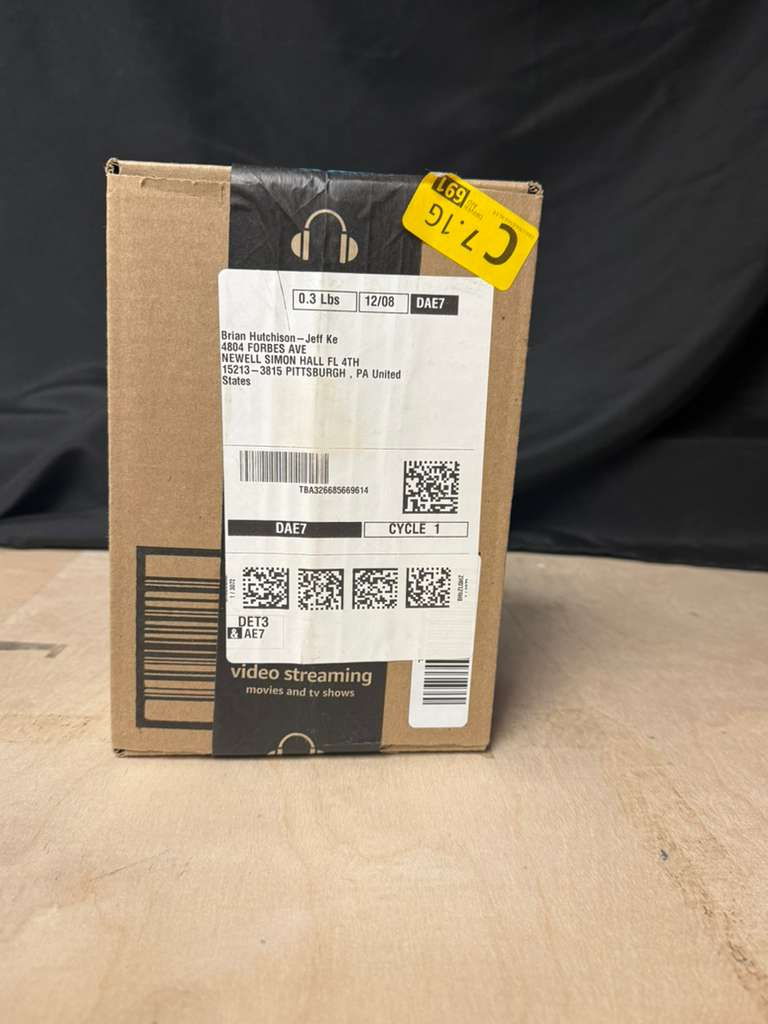
\includegraphics[width=0.24\textwidth]{objects/cardboard_box.jpeg}\hfill
    
\includegraphics[width=0.24\textwidth]{objects/cheez_it_box.jpeg}

    \vspace{0.5em}

    % Row 2
    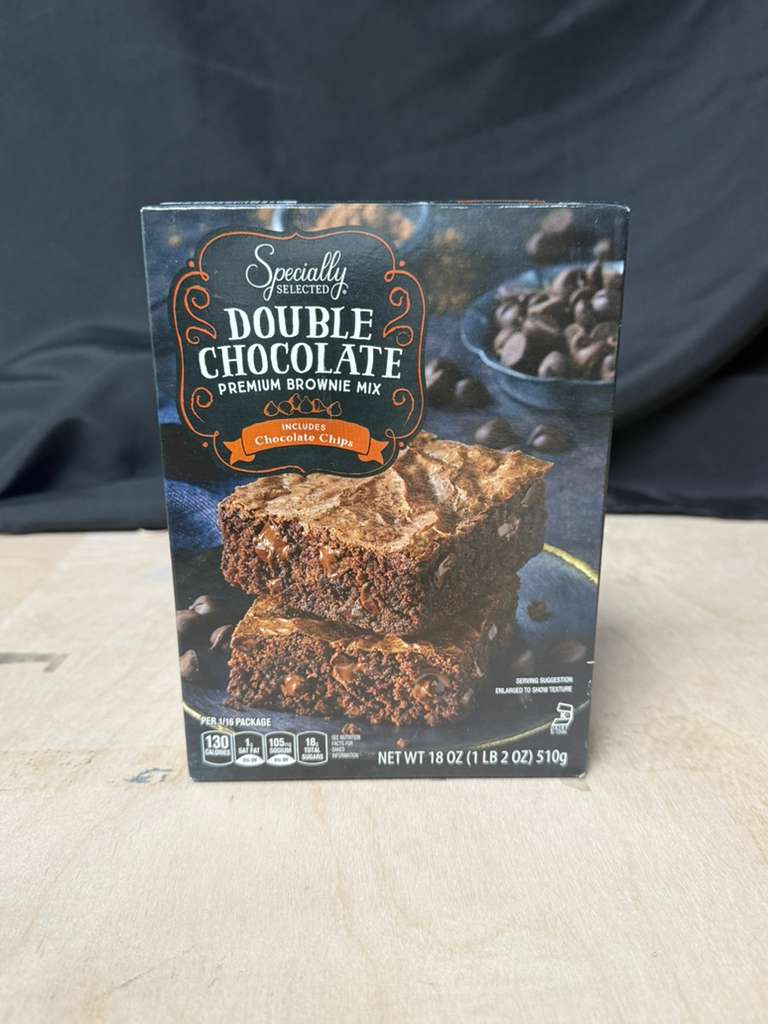
\includegraphics[width=0.24\textwidth]{objects/brownie_box.jpeg}\hfill
    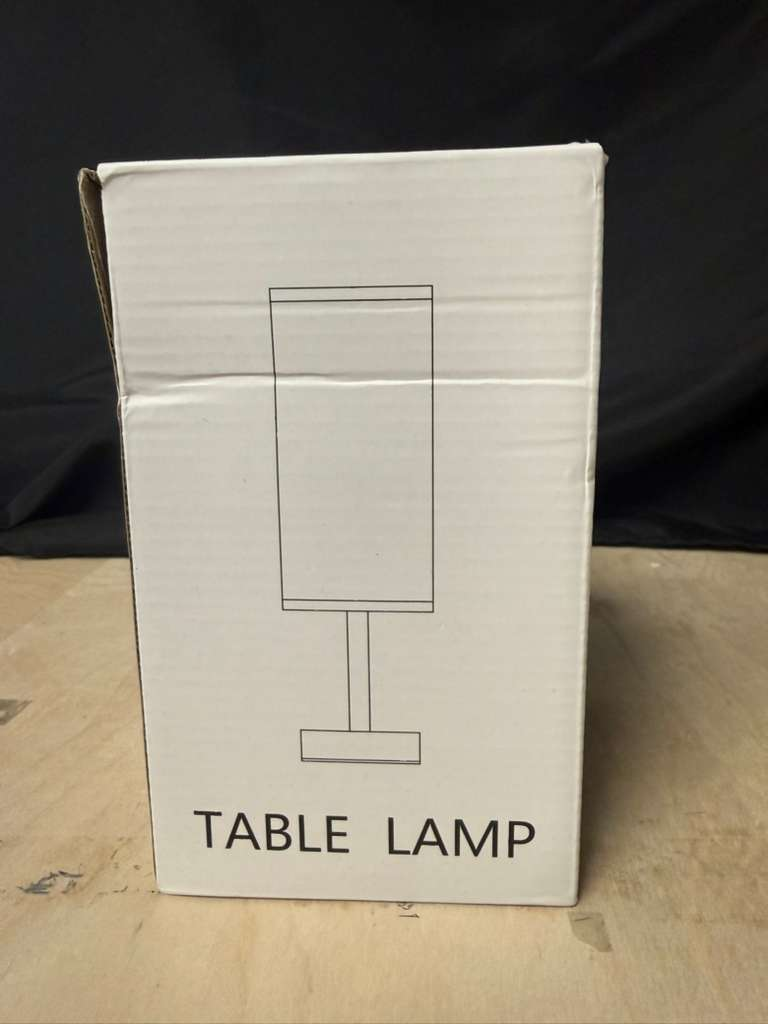
\includegraphics[width=0.24\textwidth]{objects/lamp_box.jpeg}\hfill
    
\includegraphics[width=0.24\textwidth]{objects/cake_box.jpeg}\hfill
    
\includegraphics[width=0.24\textwidth]{objects/protein_bar_2.jpeg}

    \caption{Real World Boxes}
    \label{fig:dataset}
\end{figure*}
\begin{thebibliography}{9}

\begin{figure}[h]
    \centering
    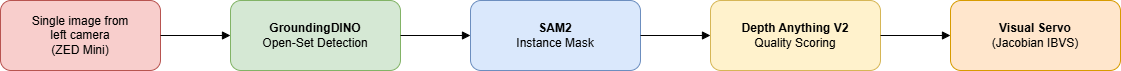
\includegraphics[width=0.45\textwidth]{visual_servo.png}
   
    \caption{Servo Pipeline using different localization methods}
    \label{fig:two_images}
\end{figure}

\begin{figure}[h]
    \centering
    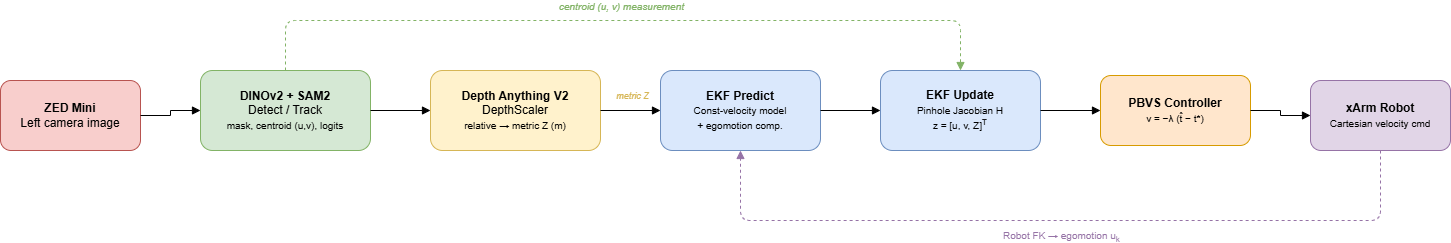
\includegraphics[width=0.45\textwidth]{visual_servo_ekf.png}
   
    \caption{Servo Pipeline using different localization methods}
    \label{fig:two_images}
\end{figure}


\bibitem{foundationpose} B. Wen, W. Yang, J. Kautz, and S. Birchfield, ``FoundationPose: Unified 6D Pose Estimation and Tracking of Novel Objects,'' in \textit{Proc. IEEE/CVF CVPR}, 2024.

\bibitem{cadena2016} C. Cadena et al., ``Past, Present, and Future of Simultaneous Localization and Mapping: Toward the Robust-Perception Age,'' \textit{IEEE Trans. Robotics}, vol. 32, no. 6, pp. 1309--1332, 2016.

\bibitem{thrun2005} S. Thrun, W. Burgard, and D. Fox, \textit{Probabilistic Robotics}. MIT Press, 2005.

\bibitem{chaumette2006} F. Chaumette and S. Hutchinson, ``Visual Servo Control, Part I: Basic Approaches,'' \textit{IEEE Robotics and Automation Magazine}, vol. 13, no. 4, pp. 82--90, 2006.

\bibitem{tao2026perceptioncontrol}
A. Tao, J. Yang, S. Oparnica, and W. Xue, ``Perception-Control Coupled Visual Servoing for Textureless Objects Using Keypoint-Based EKF,'' arXiv preprint arXiv:2602.06834, 2026.


\end{thebibliography}




\end{document}
